Pájení je jednou z mnoha možností spojování kovů. V elektronice se jedná o nejčastější možnost spojování součástek s vodivým motivem DPS. Kvalita pájeného spoje má významný vliv na spohlivost elektronických sestav a proto je potřeba věnovat její kontrole dostatečnou pozornost.

\subsection{Pájení přetavením}
Při pájení přetavením se používá pájecí pasta, která se nanáší na desku s SMD součástkami. Substrát s pastou se vloží do přetavovací pece s přesně regulovaným teplotním profilem. Teplotní profil určuje doporučenou teplotní závislost na čase pro danou pájecí pastu. Skládá se typycky z fáze předehřevu, třatavení a chlazení. Příklad teplotního profilu se nachází na obr.~\ref{fig:profil.png}.

\begin{figure}[h!]
    \centering
    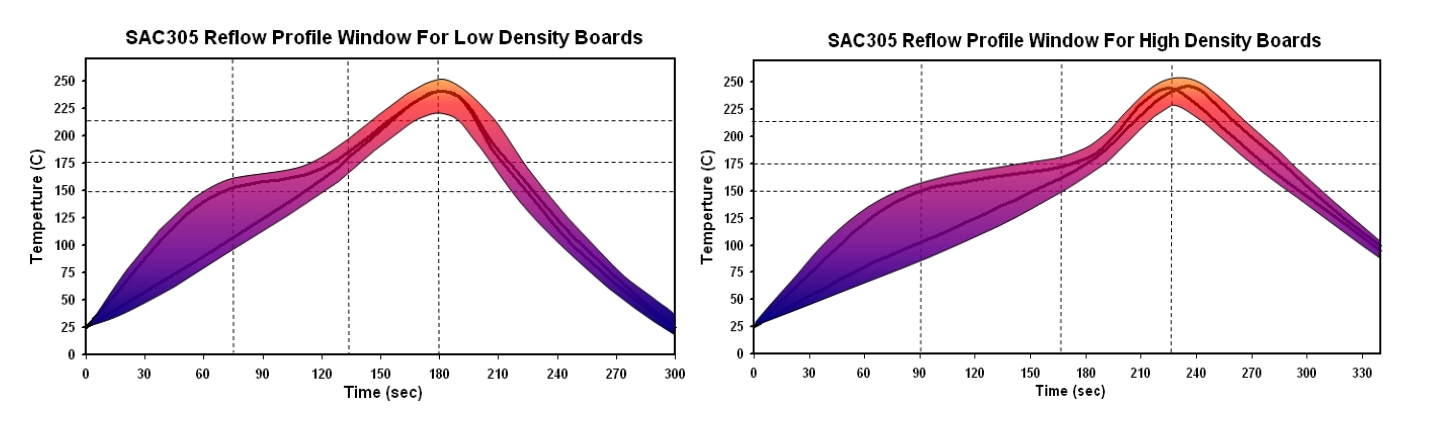
\includegraphics[width=\textwidth]{profil.png}
    \caption{Příklad teplotního profilu pro pájecí pastu WS483 (SAC 305), převzato z \cite{aimsolder_datasheet}}
    \label{fig:profil.png}
\end{figure}

\subsection{Pájení vlnou}
    Alternativou pro reflow pájení je pájecí vlna. Při pájení vlnou je potřeba využít lepidlo k upevnění součástek, které následně definovanou rychlostí a pod definovaným úhlem projedou vlnou roztavené pájky. Vlnu je možné realizovat také lokálně pro menší část DPS, kde dává tato metoda větší smysl, obecně přináší oproti reflow pájení totiž spíše nevýhody v podobě vyšší energetické náročnosti, vyšší spotřebě pájky, nutnosti použití lepidla, které zároveň znesnadňuje opravy. Také není možné tímto způsobem pájet všechny součástky a je potřeba ošetřit otvory krycí vrstvou, aby nedoško k dostání pájky na druhou stranu DPS. 

\subsection{Leaching (Odsmáčení)}
    Leaching je nežádoucí jev, při kterém dojde k odsmáčení části vodivého motivu do pájky. Pravděpodobnost tohoto jevu je dána zejména použitými materiály, také však např. jejich stářím. Pravděpodobnost zvýšíme také příliš vysokou teplotou při procesu pájení a jejím zbytečně dlouhým působením  \cite{zadani}. U pájení na tlusté vstvě je tento jev o něco častější, než u klasických DPS, protože obvykle používaný stříbrný vodivý motiv se v pájce rozpouští mnohem snáze než motiv měděný.



